\documentclass[dvipsnames,aspectratio=169,pdftex]{beamer}
\usepackage{agda}
\usepackage{stmaryrd}
\usepackage{xcolor}
\usepackage{txfonts}

\usetheme{Madrid}

\title{Towards Tagless Interpretation of Finitely Stratified System F}
\subtitle{Extended Abstract}

\author[Thiemann, Weidner]
{
\textbf{Peter Thiemann} \and
{Marius Weidner} 
}
\institute{University of Freiburg, Germany
}
\date{September 4, 2023 (TyDe, Seattle, WA, USA)}


\AtBeginSection[]{%
  \begin{frame}<beamer>
    \frametitle{Outline}
    \tableofcontents[currentsection]%[sectionstyle=show/show,subsectionstyle=hide/show/hide]
  \end{frame}
  \addtocounter{framenumber}{-1}% If you don't want them to affect the slide number
}

\usepackage{dsfont}
\usepackage{newunicodechar}
\newunicodechar{λ}{\ensuremath{\mathnormal\lambda}}
\newunicodechar{σ}{\ensuremath{\mathnormal\sigma}}
\newunicodechar{τ}{\ensuremath{\mathnormal\tau}}
\newunicodechar{π}{\ensuremath{\mathnormal\pi}}
\newunicodechar{ℕ}{\ensuremath{\mathbb{N}}}
\newunicodechar{∷}{\ensuremath{::}}
\newunicodechar{≡}{\ensuremath{\equiv}}
\newunicodechar{≅}{\ensuremath{\cong}}
\newunicodechar{∀}{\ensuremath{\forall}}
\newunicodechar{ᴸ}{\ensuremath{^L}}
\newunicodechar{ᴿ}{\ensuremath{^R}}
\newunicodechar{ʳ}{\ensuremath{^r}}
\newunicodechar{ⱽ}{\ensuremath{^V}}
\newunicodechar{⟧}{\ensuremath{\rrbracket}}
\newunicodechar{⟦}{\ensuremath{\llbracket}}
\newunicodechar{⊤}{\ensuremath{\top}}
\newunicodechar{⊥}{\ensuremath{\bot}}
\newunicodechar{₁}{\ensuremath{_1}}
\newunicodechar{₂}{\ensuremath{_2}}
\newunicodechar{₃}{\ensuremath{_3}}
\newunicodechar{₄}{\ensuremath{_4}}
\newunicodechar{₅}{\ensuremath{_5}}
\newunicodechar{₆}{\ensuremath{_6}}
\newunicodechar{₇}{\ensuremath{_7}}
\newunicodechar{₈}{\ensuremath{_8}}
\newunicodechar{₉}{\ensuremath{_9}}
\newunicodechar{∈}{\ensuremath{\in}}
\newunicodechar{₀}{\ensuremath{_0}}
\newunicodechar{′}{\ensuremath{'}}
\newunicodechar{ˢ}{\ensuremath{^S}}
\newunicodechar{ᴬ}{\ensuremath{^A}}
\newunicodechar{∘}{\ensuremath{\circ}}
\newunicodechar{𝟙}{\ensuremath{\mathds{1}}}  
\newunicodechar{𝟘}{\ensuremath{\mathds{O}}}
% \newunicodechar{𝟙}{\ensuremath{\mathbb{I}}}  
% \newunicodechar{𝟘}{\ensuremath{\mathbb{O}}}
\newunicodechar{ᴾ}{\ensuremath{^P}}
\newunicodechar{ᵀ}{\ensuremath{^T}}
\newunicodechar{⊎}{\ensuremath{\uplus}}
\newunicodechar{ι}{\ensuremath{\iota}}
\newunicodechar{⇐}{\ensuremath{\Leftarrow}}
\newunicodechar{⇒}{\ensuremath{\Rightarrow}}
\newunicodechar{∎}{\ensuremath{\mathnormal\blacksquare}}
\newunicodechar{➙}{\ensuremath{\to^P}}
\newunicodechar{Δ}{\ensuremath{\Delta}}
\newunicodechar{∅}{\ensuremath{\emptyset}}
\newunicodechar{⁺}{\ensuremath{^+}}
\newunicodechar{𝕏}{\ensuremath{\mathbb{X}}}
%\newunicodechar{·}{\ensuremath{\cdot}} %seems to be defined already!
\newunicodechar{∙}{\ensuremath{\bullet}}
\newunicodechar{⁇}{\ensuremath{?}}
\newunicodechar{‼}{\ensuremath{!}}
\newunicodechar{⊕}{\ensuremath{\oplus}}
\newunicodechar{ℤ}{\ensuremath{\mathbb{Z}}}
\newunicodechar{μ}{\ensuremath{\mu}}
\newunicodechar{∃}{\ensuremath{\exists}}
\newunicodechar{⨟}{\ensuremath{\fatsemi}}
\newunicodechar{Σ}{\ensuremath{\Sigma}}
\newunicodechar{ᵣ}{\ensuremath{_r}}
\newunicodechar{ᵢ}{\ensuremath{_i}}
\newunicodechar{≢}{\ensuremath{\nequiv}}
\newunicodechar{≟}{\ensuremath{\stackrel{{\tiny?}}{=}}}
\newunicodechar{≤}{\ensuremath{\le}}
\newunicodechar{ᵇ}{\ensuremath{^b}}
\newunicodechar{𝓣}{\ensuremath{\mathcal{T}}}
\newunicodechar{𝓔}{\ensuremath{\mathcal{E}}}
\newunicodechar{Γ}{\ensuremath{\Gamma}}
\newunicodechar{γ}{\ensuremath{\gamma}}
\newunicodechar{⊔}{\ensuremath{\sqcup}}
\newunicodechar{α}{\ensuremath{\alpha}}
\newunicodechar{η}{\ensuremath{\eta}}
\newunicodechar{ω}{\ensuremath{\omega}}
\newunicodechar{◁}{\ensuremath{\lhd}}
%PT: seems to be already defined
%\newcommand{\lambdabar}{{\mkern0.75mu\mathchar '26\mkern -9.75mu\lambda}}
\newunicodechar{ƛ}{\ensuremath{\lambdabar}}
\newunicodechar{Λ}{\ensuremath{\mathnormal\Lambda}}
\newunicodechar{ρ}{\ensuremath{\rho}}
\newunicodechar{𝓖}{\ensuremath{\mathcal{G}}}
\newunicodechar{ℓ}{\ensuremath{\ell}}
\newunicodechar{♯}{\ensuremath{\sharp}}
\newunicodechar{⇓}{\ensuremath{\Downarrow}}
\newunicodechar{𝓥}{\ensuremath{\mathcal{V}}}
\newunicodechar{∧}{\ensuremath{\wedge}}
\newunicodechar{ₛ}{\ensuremath{_s}}
\newunicodechar{χ}{\ensuremath{\chi}}
\newunicodechar{⊨}{\ensuremath{\models}}
\newunicodechar{⦂}{\ensuremath{\mathbf{:}}}
\newunicodechar{ς}{\ensuremath{\varsigma}}
\newunicodechar{𝓓}{\ensuremath{\mathcal{D}}}
\newunicodechar{∎}{\ensuremath{\square}}
\newunicodechar{■}{\ensuremath{\blacksquare}}
\newunicodechar{↠}{\ensuremath{\twoheadrightarrow}}
\newunicodechar{↪}{\ensuremath{\hookrightarrow}}
\newunicodechar{β}{\ensuremath{\beta}}
\newunicodechar{ξ}{\ensuremath{\xi}}
\input{latex/Tagless-final}

\begin{document}
\begin{frame}{\null}
  \titlepage 
\end{frame}
\begin{frame}
  \frametitle{Types of System F}
  \framesubtitle{Intrinsically scoped encoding}
  \SFType
  \begin{itemize}
  \item Polymorphic lambda calculus (Girard, Reynolds)
  \item Impredicative: quantification extends over all types
  \item In $T = \forall \alpha.S$, $\alpha$ ranges over all types including $T$
  \item Precludes a set-theoretic semantics
  \end{itemize}
\end{frame}
\begin{frame}
  \begin{center}
    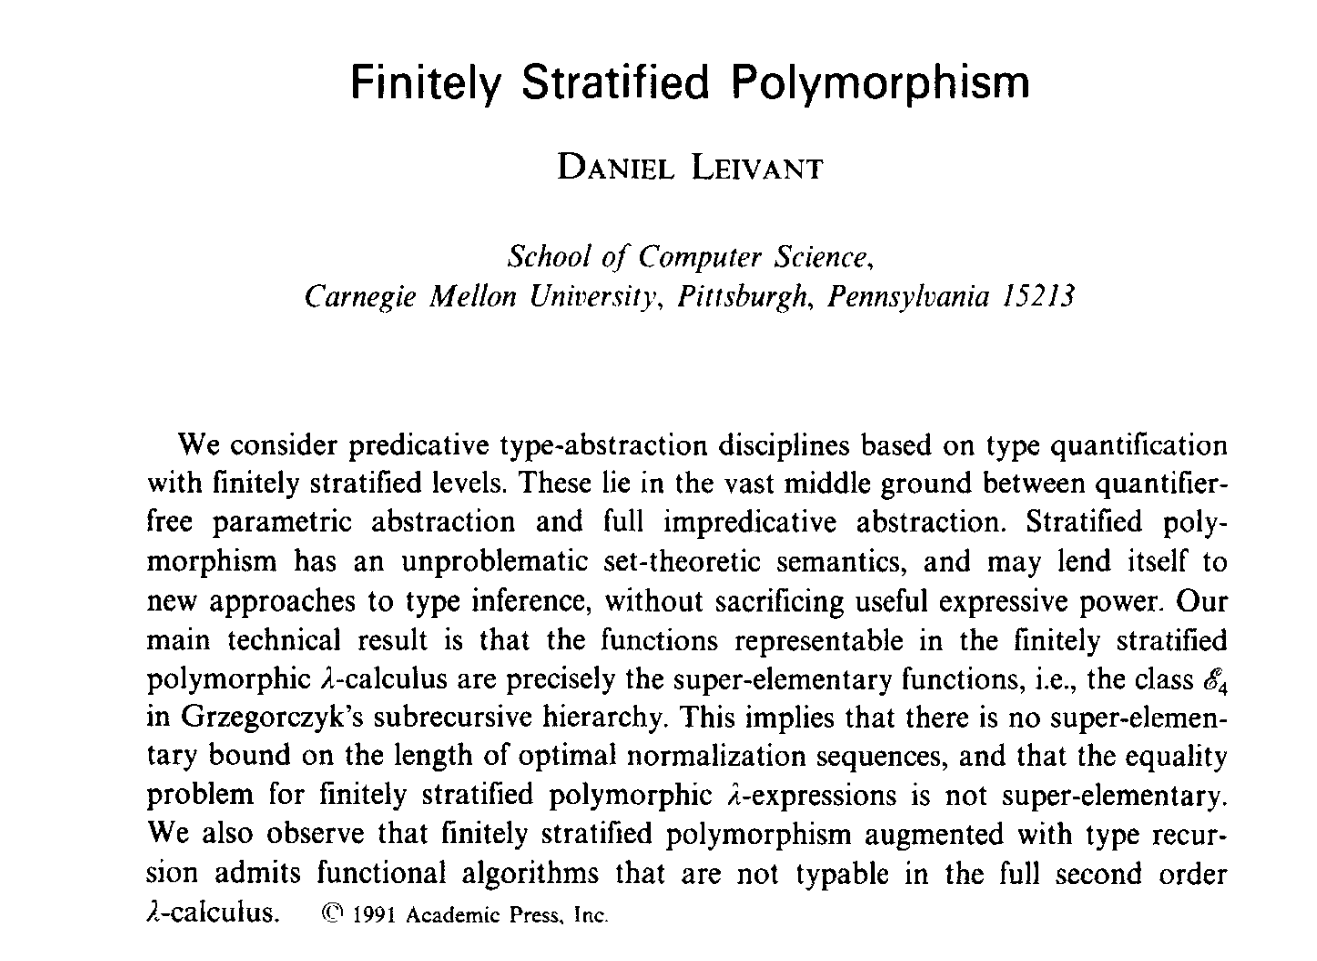
\includegraphics[scale=0.25]{images/FinitelyStratifiedPolymorphism.png}
  \end{center}
\end{frame}
\begin{frame}
  \frametitle{Finite Stratification}
  \framesubtitle{Intrinsically leveled encoding}
  \begin{itemize}
  \item Each type has a level (i.e., a natural number)
  \item Quantification is only possible over types at lower level
  \item Predicativity is retained
  \item Simple set-theoretic semantics
  \end{itemize}
  \pause
  \TFType
  \pause\vspace{-2\baselineskip}
  \TFlevel
\end{frame}
\begin{frame}
  \frametitle{Semantics of Types}
  \begin{itemize}
  \item Leivant's levels correspond to Agda's universe levels, so \dots
  \end{itemize}
  \pause
  \TFTEnvP
  \pause\vspace{-2\baselineskip}
  \TFTSemP
  \begin{itemize}
  \item Works because we're using \AgdaFunction{Level} in the syntax!
  \end{itemize}
\end{frame}
\begin{frame}
  \frametitle{Type Environments and Variables}
  \begin{itemize}
  \item A single environment for type and term variables
  \item Encoding inspired by \emph{System F in Agda, for fun and profit} (Chapman et al, MPC 2019)
  \end{itemize}
  \TFTVEnv
  \pause\vspace{-2\baselineskip}
  \TFCleanerinn
\end{frame}
\begin{frame}
  \frametitle{Syntax of Expressions (Excerpt)}
  \framesubtitle{Intrinsically typed encoding}
  \TFCleanExpr
\end{frame}
\begin{frame}
  \frametitle{Set-Theoretic Semantics of Expressions}
  \TFExprSem
  where
  \TFVEnv
\end{frame}
\begin{frame}
  \frametitle{Set woes}
  \begin{itemize}
  \item \AgdaFunction{Setω} is Agda's sort that contains \AgdaFunction{Set ℓ}, for all \AgdaFunction{ℓ}.
  \item Some proofs argue about equality in types of sort \AgdaFunction{Setω}:
    \TFSingleSubstPreserves
  \item This equality is easy to define, but leads to a proliferation of uninteresting copies of library functions like \AgdaFunction{cong}, \AgdaFunction{subst}, \dots; equational reasoning; extensionality axioms, and so on.
  \end{itemize}
\end{frame}
\begin{frame}
  \frametitle{Set woes II}
  \begin{itemize}
  \item Consider extending the calculus with level-polymorphism.
  \item Can be modeled in Agda, but forces a departure from the simple semantics of types.
  \item A level-polymorphic function is a member of \AgdaFunction{Setω}, but that means the semantics of a type can no longer be in  \AgdaFunction{Setω}!
  \item It must be in \AgdaFunction{Setω₁} $\Longrightarrow$ can't index types by levels, need more equalities, and so on.
  \end{itemize}
  \begin{exampleblock}{Wish to the  Agda maintainers}
    \begin{itemize}
    \item Extend \AgdaFunction{Level} to include a larger subset of ordinals.
    \item Leivant's 1989 paper \emph{Stratified Polymorphism} suggests
      a useful subset.
    \item Recent work by Bezem, Coquand, Dybjer, Escardo (TYPES 2022)
    \end{itemize}
  \end{exampleblock}
\end{frame}
\begin{frame}
  \frametitle{Where do we go from here?}
  \begin{itemize}
  \item All results for Stratified System F apply directly to subsystems like ML.
  \item Intrinsically typed small-step and big-step semantics.
  \item Soundness with respect to denotational semantics (stratification required).
  \item Logical relation and adequacy (stratification required).
  \end{itemize}
\end{frame}
\end{document}
